% Couverture, page de titre et page des crédits.
% L'image de couverture est calculée par code/cover.py (cellules de Voronoï du réseau triangulaire).
\thispagestyle{empty}
\begin{tikzpicture}[remember picture,overlay]
  \node[inner sep=0pt] at (current page.center)
    {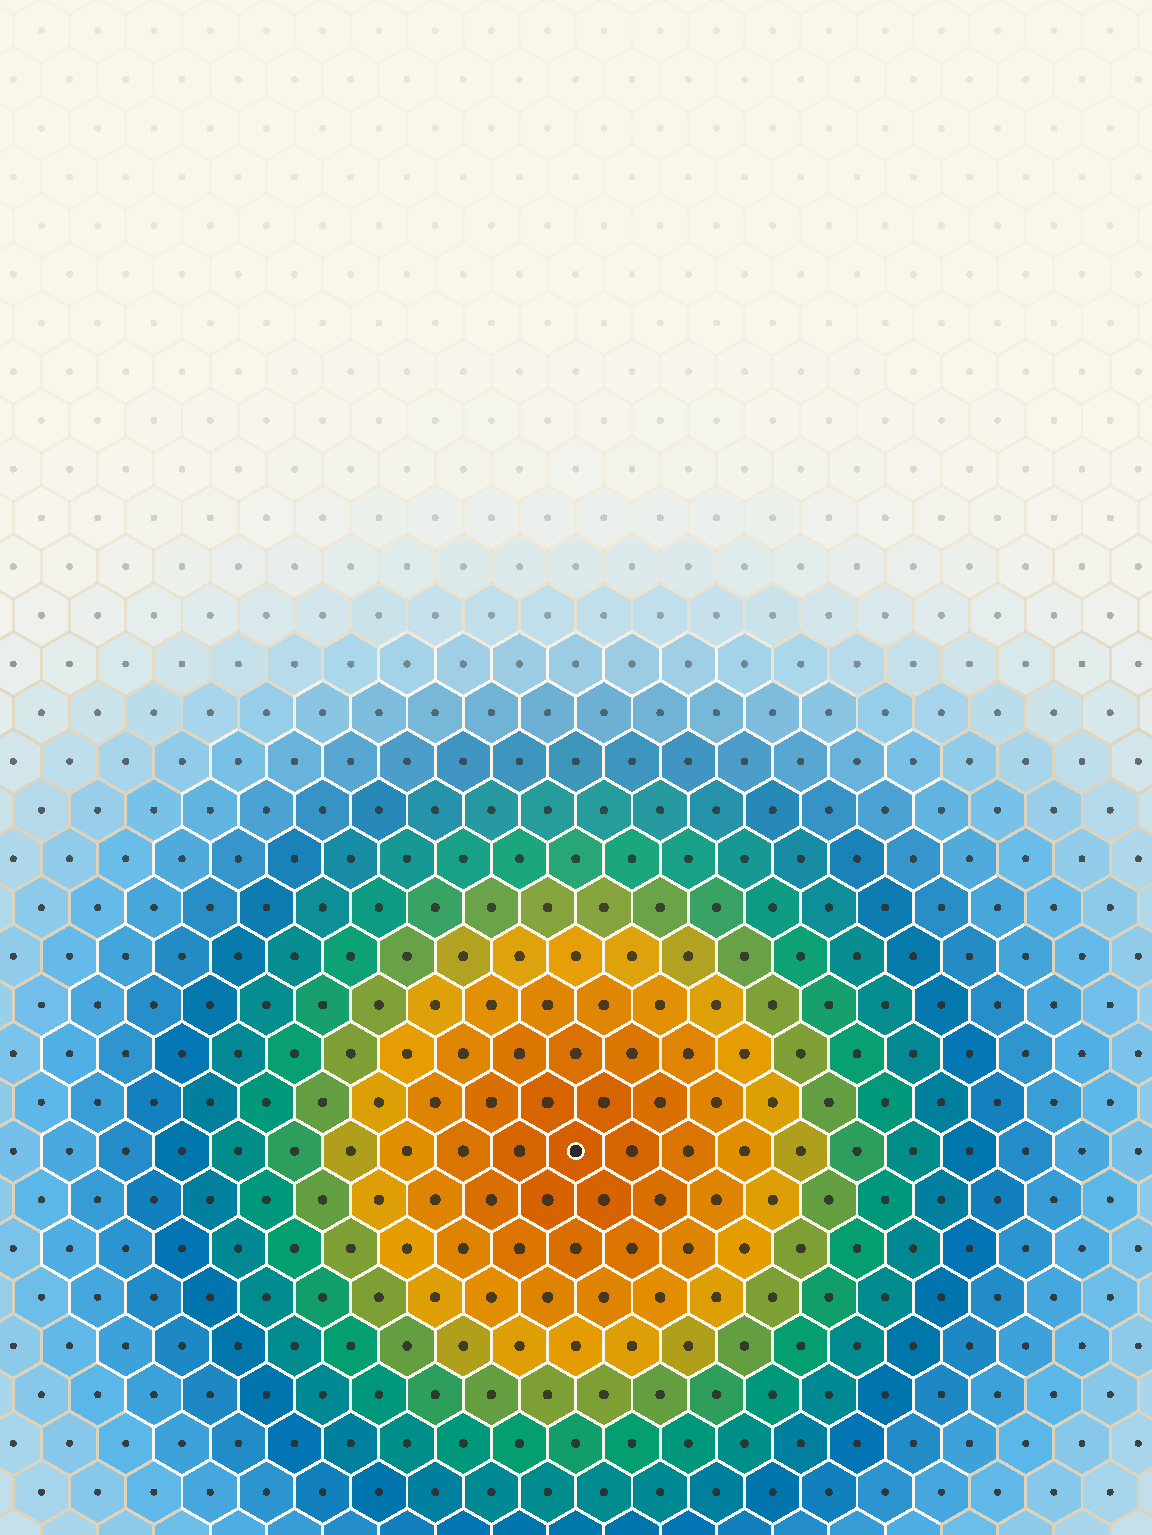
\includegraphics[width=\paperwidth,height=\paperheight]{cover.pdf}};
  \node[anchor=north west,inner sep=0pt,text width=15.2cm,align=left]
    at ([xshift=2.1cm,yshift=-3.0cm]current page.north west) {%
    {\sffamily\bfseries\footnotesize\color{okbleu}\textls[200]{XAVIER CALLENS}}\\[1.1cm]
    {\fontsize{40}{44}\selectfont\color{encre}Le\hspace{0.3em}journal\\[2pt] des\hspace{0.3em}découvertes}\\[0.8cm]
    {\color{okorange}\rule{3.2cm}{1.6pt}}\\[0.55cm]
    {\fontsize{13.5}{18}\selectfont\itshape\color{encre!85}Une année où l'IA propose, l'ordinateur calcule,\\
      la preuve juge et l'humain décide du sens}};
  \node[anchor=south west,inner sep=0pt,text width=15cm,align=left]
    at ([xshift=2.1cm,yshift=1.6cm]current page.south west) {%
    {\sffamily\footnotesize\bfseries\color{ivoire}\textls[160]{SOCRATEAI LAB}}};
\end{tikzpicture}
\clearpage
% verso de la couverture
\thispagestyle{empty}
\vspace*{\fill}
\begin{adjustwidth}{0pt}{-3cm}
\noindent{\footnotesize\color{encre!70}\textit{La couverture.} Chaque hexagone est la cellule de Voronoï d'un point du
réseau triangulaire de densité~1 : l'ensemble des endroits du plan plus proches de ce point que de tout autre. Toutes
ces cellules ont exactement la même aire, égale à~1. La couleur d'une cellule donne le poids
$e^{-\pi\alpha r^2}$, avec $\alpha=0{,}009$, de son point dans l'énergie du point central (le point noir), où $r$ est
la distance qui les sépare : vermillon et orange tout près, puis vert et bleu, ivoire au loin. L'image est calculée, pas dessinée à la
main (\texttt{code/cover.py}) ; le script vérifie que chaque cellule a bien six côtés et une aire de~1, et qu'un
réseau légèrement déformé échoue à ce test.}
\end{adjustwidth}
\clearpage

% page de titre
\thispagestyle{empty}
\vspace*{2.2cm}
{\sffamily\bfseries\footnotesize\color{okbleu}\textls[200]{XAVIER CALLENS}}\par
\vspace{1.4cm}
{\fontsize{34}{38}\selectfont Le\hspace{0.3em}journal des\hspace{0.3em}découvertes\par}
\vspace{0.6cm}
{\color{okorange}\rule{3.2cm}{1.6pt}}\par
\vspace{0.5cm}
{\large\itshape Une année où l'IA propose, l'ordinateur calcule,\\ la preuve juge et l'humain décide du sens\par}
\vspace{1.4cm}
{\normalsize Vingt contributions en mathématiques, physique, génétique et cosmologie,\\
racontées en mots simples, avec leurs limites et leurs erreurs\par}
\vspace*{\fill}
{\sffamily\footnotesize\color{encre!80}\textls[120]{SOCRATEAI LAB}\quad·\quad\lfstyle Version 1, octobre 2026\par}
\clearpage

% verso : crédits et déclaration sur l'IA
\thispagestyle{empty}
\vspace*{\fill}
\begin{adjustwidth}{0pt}{-2cm}
\small
\noindent\textbf{Le journal des découvertes.} Une année où l'IA propose, l'ordinateur calcule, la preuve juge et
l'humain décide du sens.\par\medskip
\noindent Xavier Callens, SocrateAI Lab. Version 1, octobre 2026. DOI~: 10.5281/zenodo.23669395.\par\medskip
\noindent\textbf{Déclaration sur l'intelligence artificielle.} Ce livre a été rédigé avec des agents d'intelligence
artificielle (Claude, d'Anthropic), sous la direction de l'auteur, qui en a choisi le sujet, le plan et le ton, et qui
en porte la responsabilité. Les résultats qu'il raconte ont eux aussi été produits par des agents d'IA sous la
direction de l'auteur, puis audités par d'autres agents d'IA. \textbf{Aucun mathématicien humain ne les a relus.}
Plusieurs d'entre eux dépendent de théorèmes publiés par openai/math, eux aussi produits par une IA et non encore
évalués par des pairs. Chaque affirmation porte un niveau de confiance (A, As, L, C ou X), expliqué au chapitre~1.\par\medskip
\noindent\textbf{Sources.} Les faits et les nombres de ce livre viennent des dossiers des travaux eux-mêmes
(Zenodo, GitHub) et du dossier de sélection décrit à la fin du livre (« Comment ce livre a été fabriqué »). Un nombre
qui n'y figure pas n'est pas utilisé.\par\medskip
\noindent\textbf{Composition.} \LaTeX{} (pdflatex), polices Cochineal et Source Sans Pro, palette de couleurs
Okabe--Ito, choisie pour rester lisible par les personnes daltoniennes. Les figures sont calculées par des
programmes à partir des nombres réels.
\end{adjustwidth}
\vspace*{1.5cm}
\clearpage
